\begin{figure}[!htb]
  \centering
  \begin{minipage}[t]{0.48\linewidth}
    \centering
    {\small\textbf{(a)} The zero-tilt geometry, $\eps=0$}\par\smallskip
    \begin{tikzpicture}[x=0.205\linewidth,y=0.205\linewidth,
      font=\scriptsize,line cap=round,line join=round]
      \coordinate (A) at (-1.8,0.4);   %
      \coordinate (B) at (1.8,-0.4);   %
      \coordinate (C) at (-0.95,2.45); %
      \coordinate (D) at (0.95,3.35);  %
      \coordinate (AC) at (-1.375,1.425);
      \coordinate (BC) at (0.425,1.025);
      \coordinate (BD) at (1.375,1.475);
      \coordinate (AD) at (-0.425,1.875);
      \fill[black!3] (A)--(B)--(D)--(C)--cycle;
      \draw[black!45,densely dashed] (A)--(D);
      \fill[blue!9] (AC)--(BC)--(BD)--(AD)--cycle;
      \draw[black!55,thin] (AC)--(BC)--(BD)--(AD)--cycle;
      \draw[black!65] (A)--(C)--(D)--(B)--cycle (B)--(C);
      \draw[blue!65!black,very thick] (A)--(B);
      \draw[orange!80!black,very thick] (C)--(D);
      \draw[->,blue!65!black,thick] (-1.121,0.821)--(0.931,0.365);
      \draw[->,blue!65!black,thick] (-0.679,1.232)--(0.869,0.888);
      \draw[->,orange!80!black,thick] (-0.352,1.970)--(0.712,2.474);
      \draw[->,orange!80!black,thick] (-0.5885,1.8185)--(0.2285,2.2055);
      \node[blue!65!black,anchor=north] at (0.48,0.35) {$x$};
      \node[orange!80!black,anchor=south west] at (0.70,2.48) {$y$};
      \node[fill=white,inner sep=1.3pt] at (0,1.44) {$t=\tfrac12$};
      \node at (-1.50,-0.13) {$(-1,0,0)$};
      \node at (1.50,-0.83) {$(1,0,0)$};
      \node at (-1.44,2.94) {$(0,-1,H)$};
      \node at (1.04,3.81) {$(0,1,H)$};
      \path[use as bounding box] (-2.38,-0.99) rectangle (2.38,4.00);
    \end{tikzpicture}\par
    {\scriptsize Physical coordinates $(x,y,Ht)$; $H=\sqrt{2}$.}
  \end{minipage}\hfill
  \begin{minipage}[t]{0.49\linewidth}
    \centering
    {\small\textbf{(b)} Matching after the tilt, $x=X$}\par\smallskip
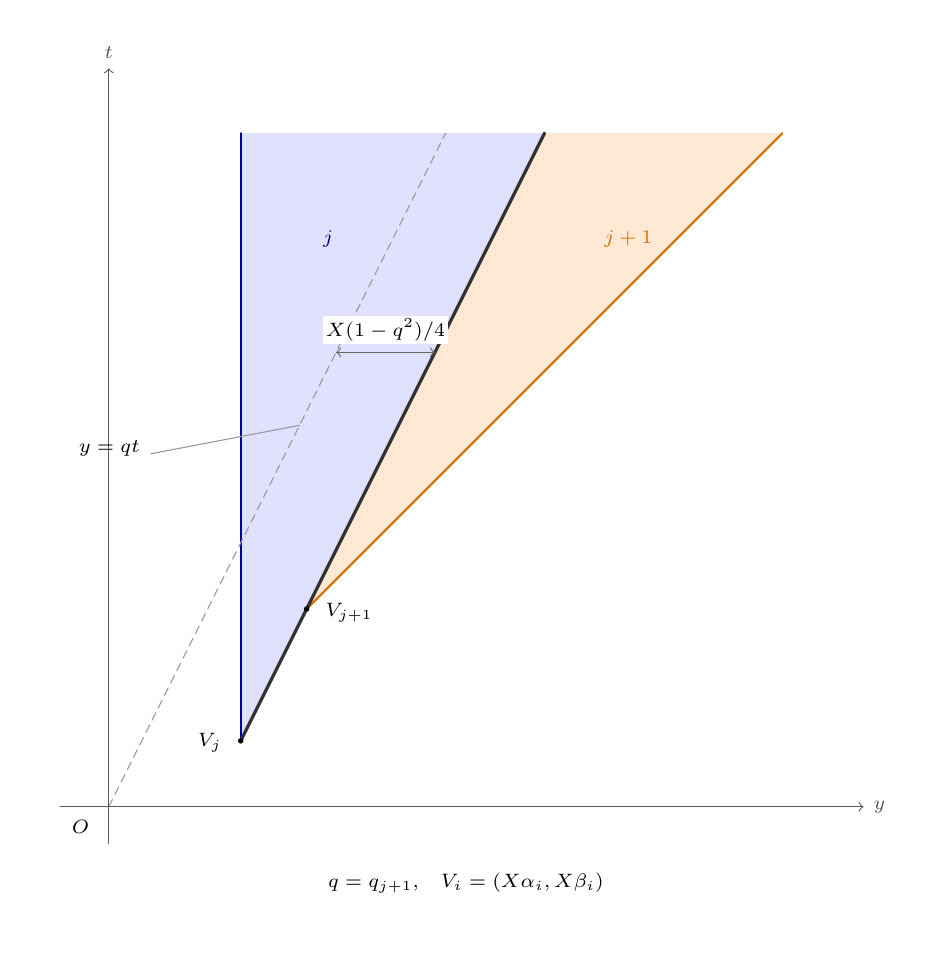
\begin{tikzpicture}[x=0.85\linewidth,y=0.85\linewidth,
  font=\scriptsize,line cap=round,line join=round]
  \coordinate (A) at (.1625,.08125);
  \coordinate (B) at (.24375,.24375);
  \coordinate (Ltop) at (.1625,.83);
  \coordinate (Mtop) at (.536875,.83);
  \coordinate (Rtop) at (.83,.83);
  \fill[blue!12] (A)--(Ltop)--(Mtop)--cycle;
  \fill[orange!17] (B)--(Mtop)--(Rtop)--cycle;
  \draw[blue!65!black,thick] (A)--(Ltop);
  \draw[orange!85!black,thick] (B)--(Rtop);
  \draw[black!80,very thick] (A)--(Mtop);
  \draw[black!40,densely dashed] (0,0)--(.415,.83);
  \draw[<->,black!60] (.28,.56)--(.401875,.56);
  \node[fill=white,inner sep=1pt,anchor=south] at (.3409375,.57)
    {$\eps X(1-q^2)/4$};
  \draw[->,black!65] (-.06,0)--(.93,0) node[right] {$y$};
  \draw[->,black!65] (0,-.045)--(0,.91) node[above] {$t$};
  \node[anchor=north east] at (-.012,-.005) {$O$};
  \fill (A) circle[radius=1pt];
  \fill (B) circle[radius=1pt];
  \node[anchor=east] at (.151,.079) {$V_j$};
  \node[anchor=west] at (.255,.239) {$V_{j+1}$};
  \node[blue!65!black] at (.27,.70) {$j$};
  \node[orange!85!black] at (.64,.70) {$j+1$};
  \node[anchor=south east,align=right] at (.05,.42) {$y=qt$};
  \draw[black!40,thin] (.052,.435)--(.235,.47);
  \node[anchor=north,align=center] at (.44,-.07)
    {$q=q_{j+1}$,\quad $V_i=(\eps X\alpha_i,\eps X\beta_i)$};
  \path[use as bounding box] (-.10,-.15) rectangle (1,.96);
\end{tikzpicture}\par
{\scriptsize The common supporting line is $y=qt+\eps X(1-q^2)/4$.}

  \end{minipage}
  \caption{(a) At zero tilt, cylinders parallel to the two opposite edges cover the lower and upper halves of $K$.
  (b) In the plane $x=X$, neighboring angular sectors have distinct translated vertices $V_j$ and $V_{j+1}$, but their sides at $q=q_{j+1}$ lie on the same line $y=qt+\eps X(1-q^2)/4$.
  The dashed line is $y=qt$, its zero-tilt position. Tilt and sector widths are exaggerated. Radial cutoffs are omitted; the colored regions end at the boundary of the displayed window.}
  \label{fig:construction}
\end{figure}
